\chapter{开发工具及相关技术介绍}

\section{开发工具介绍}
    \subsection{Scala}
        Scala(Scalable Language)是一门多范式的编程语言,集成了面向对象编程、函数式编程和命令式编程的各种特性,同时该语言基于JVM,兼容Java编写的工具包,同时其内置的静态类型极大程度上降低了构建高性能系统的难度,是一门十分灵活、高级的编程语言。
        Scala自2004年被设计出来以后不断发展壮大,截止2019年2月已经发展到2.12.8版本,社区十分活跃,功能十分强大,不断的被大厂应用于产品:
        \begin{itemize}[topsep = 0 pt]
            \setlength{\topsep}{0pt}
            \setlength{\itemsep}{0pt}
            \setlength{\parsep}{0pt}
            \setlength{\parskip}{0pt}
            \setlength{\partopsep}{0pt}
            \item  Twitter宣布他们已经把大部分后端程序从Ruby迁移到Scala
            \item  Wattzon已经公开宣称,其整个平台都已经是基于Scala基础设施编写的
            \item  瑞银集团把Scala用于一般产品中
            \item  Coursera把Scala作为服务器语言使用
            \item  由UCB开发的大数据集群计算平台——Spark使用Scala作为开发语言
        \end{itemize}       
        \begin{lstlisting}[title=Scala Hello world, frame=shadowbox]
object HelloWorld {
    def main(args: Array[String]) {
        println("Hello, world!")
    }
}
        \end{lstlisting}

    \subsection{Chisel3}
        Chisel(Constructing Hardware In a Scala Embedded Language)是一款由UC Berkeley开发并开源的硬件描述语言,支持高度参数化的生成器和分层设计等高级设计方法进行硬件设计。
        需要说明的是Chisel并不是将C转换成RTL(类似HLS),而是货真价实的硬件描述语言。其本身作为工具包内嵌于Scala中。 \\
        Chisel主要特性归纳如下:
        \begin{figure}[h]
            \begin{itemize}[topsep = 0 pt]
                \setlength{\topsep}{0pt}
                \setlength{\itemsep}{0pt}
                \setlength{\parsep}{0pt}
                \setlength{\parskip}{0pt}
                \setlength{\partopsep}{0pt}
                \item 支持抽象的数据类型和接口
                \item 批量连接
                \item 层次化、面向对象、函数式构造
                \item Scala元编程实现了高度参数化
                \item 内置了可配置的标准单元库
                \item 可生成Verilog
                \item 多时钟域设计
                \item 开源,完备的文档,活跃的社区
            \end{itemize}
        \end{figure}
        \begin{figure}[h]
            \label{chisel_example}
            \begin{lstlisting}[title=Chisel Example, frame=shadowbox]
import chisel3._
class MaxN(val n: Int, val w: Int) extends Module {
    private def Max2(x: UInt, y: UInt) = Mux(x > y, x, y)
    val io = IO(new Bundle {
        val ins = Input(Vec(n, UInt(w.W)))
        val out = Output(UInt(w.W))
    })
    io.out := io.ins.reduceLeft(Max2)
}
            \end{lstlisting}
        \end{figure}

    \subsection{Verilator}
Verilator是速度最快的Verilog HDL模拟器,性能优于大部分商用模拟器。其将Verilog转换为使用C++或SystemC编写的时序准确的模型。
\begin{wrapfigure}{r}{4cm}%靠文字内容的左侧
    
\includegraphics[width=4cm]{../pdf/verilator.png}\
    \caption{Verilator Logo}
\end{wrapfigure}
    Verilator专为需要快速仿真性能的大型项目而设计,尤其适用于为嵌入式软件设计团队生成可执行的CPU模型。其无法替代NC-Verilog,VCS等商业Verilog模拟器,但可以将可综合的Verilog迁移到C++或SystemC,并且是免费的。
Verilator的性能十分优秀,并不是将Verilog代码直接进行翻译而是优化为更快的线程区分模型。单线程的Verilator模型比传统Verilog仿真器(例如Icarus Verilog)快100倍,多线程可以获得额外的2倍~10倍性能。
目前Verilator已经用于仿真百万级门电路的设计中,并且被很多IP厂商支持,包括ARM和RISC-V。\\
其中Verilator官方网站给出一些与主流仿真器速度比较参考。
        \begin{itemize}[topsep = 0 pt]
            \setlength{\topsep}{0pt}
            \setlength{\itemsep}{0pt}
            \setlength{\parsep}{0pt}
            \setlength{\parskip}{0pt}
            \setlength{\partopsep}{0pt}
            \item Verilator比Icarus Verilog快90倍
            \item Verilator比ModelSim SE快10至40倍
            \item Verilator比NC-Verilog快3倍
            \item Verilator比VCS快1.5倍
        \end{itemize}


\section{异构处理器}
    \subsection{ZYNQ架构}
    ZYNQ是Xilinx于2010年4月发布的可扩展架构平台,该平台基于流行的ARM处理器结合Xilinx 28nm 7系FPGA工艺打造的SoC实现了高度的灵活性、强大的配置性和高特性的统一。
    其中可编程逻辑可由用户配置,并通过互联模块连接,可为用户提供自定义的逻辑,从而极大扩展了处理系统的性能和功能,不过和传统FPGA不同,ZYNQ不仅可以在开机时配置也可以根据需要实时进行配置。
    \begin{figure}[h]
        \label{zynq}
        \centering
        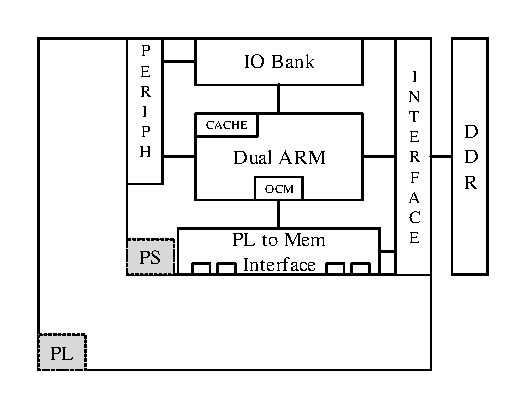
\includegraphics{../pdf/zynq.pdf}
        \caption{ZYNQ架构示意图}
        \label{}
    \end{figure}
    ZYNQ由于CPU+FPGA的架构十分契合异构计算的需求,同时PS与PL之间可以通过设计好的高带宽的AXI接口进行数据交互,开发者只需将精力集中在加速器设计和CPU数据调度上即可。
    \subsection{RISC-V}
    RISC-V从伯克利大学诞生的一款开源指令集架构,引起业界的轰动,普遍认为RISC-V可能会改变现有的由ARM、x86主导的处理器市场竞争格局。

    由于RISC-V是新的指令集架构,因此无需考虑向前兼容,没有像ARM、x86架构沉重的历史包袱,指令集的设计也更加精简。

    \begin{table}[h] %开始一个表格environment,表格的位置是h,here。  
        \label{riscv_compare}
        \centering
        \caption{RISC-V与ARM/x86比较} %显示表格的标题  
        \begin{tabular}{l|l|l} %设置了每一列的宽度,强制转换。  
        \hline  
        特性 & ARM/x86 & RISC-V \\
        \hline %画一个横线,下面的就都是一样了,这里一共有4行内容  
        架构篇幅 & 数千页  & 目前仅有300页 \\
        \hline  
        模块化 & 不支持  & 支持模块化可配置指令子集 \\
        \hline  
        可扩展性 & 不支持 & 支持扩展自定义指令 \\
        \hline  
        指令数目 & 指令多且不同分支不兼容 & 一套指令支持所有架构分支,基本指令仅40条 \\
        % \hline  
        % 易实现性 & 硬件实现十分复杂 &  \\
        \hline  
        \end{tabular}  
    \end{table}

    由伯克利大学维护的一款开源RISC-V芯片生成器Rocket-Chip-Generator,能够根据用户需要生成完整的、可综合的硬件电路,同时具备完整的工具链、准确的仿真器环境,目前已被各大厂商应用。

    \begin{figure}[h]
        \label{rocc}
        \centering
        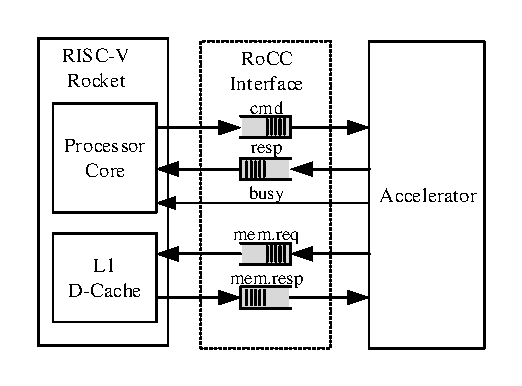
\includegraphics{../pdf/rocc.pdf}
        \caption{RoCC接口信号示意图}
        \label{}
    \end{figure}

    Rocket-Chip原生支持自定义指令集扩展,其带有一RoCC(Rocket Custom Coprocessor)接口,其协议简单、功能强大,可以十分灵活的以自定义加速器进行协同工作。
    
    \subsection{异构处理器与传统计算架构}
            \subsubsection{CPU}
            首先,CPU在深度学习计算中很重要,例如使用了16000颗CPU搭建的“Google Brain”网络,又比如1920颗CPU搭建的“AlphaGo”。如今,CPU依旧是主流深度学习平台的重要组成部分,
            但在深度学习领域,CPU在架构方面有着先天的不足,从芯片面积上看,Cache和Control单元占据了绝大部分面积,而用于计算的ALU面积却比较少;每颗核心都狠强大,但核心数量少。
            因此CPU重在数据调度,并不擅长大规模简单的运算。
            \subsubsection{GPU}
            反观GPU,虽然每颗核心都比较弱,只能完成简单的计算,但通常一个GPU都是上百上千个核心,芯片面积上用于计算的ALU单元占据了绝大部分,当所有核心都被调用起来,其运算能力远远大于CPU。
            同时,GPU普遍采用DDR5片上显存颗粒,更高的工作频率带来了更快的数据读写速度,而且总线带宽大。
            \subsubsection{异构的优势}
            目前做深度学习开发普遍采用CPU+GPU这种异构形式作为首要开发平台,既可以利用CPU强大的调度能力也可以利用GPU超快的计算速度,但这种模式是一种通用级的解决方法,应用在细分的专业领域边显的过于臃肿,不仅设备体积大,功耗也高。
            一般情况下,当模型训练完成后,需要利用模型进行推理计算,这部分不需要复杂的反向传播计算,若继续采用训练时的CPU+GPU平台,不仅造成资源浪费,量产时成本极高。
            因此针对推断,我们希望能找到一种低功耗、高性能的解决方案,因此使用FPGA和ASIC具有极大的优势。

            相比于通用的CPU+GPU的架构,CPU+FPGA/ASIC组成的异构平台具有更高的计算能效比,同时成本更低,十分适合当下嵌入式IoT领域对低功耗、高灵活性的需求。
            相比于受限于冯诺依曼架构的CPU/GPU,FPGA和ASIC在设计时可以通过多核心、流水线等技术充分发挥并行计算的特性,大大提高数据吞吐量。

\section{深度学习}
    \subsection{YOLO}
    YOLO(You only look once)是一个端到端的实时目标检测算法,不像传统的目标识别CNN模型需要训练多个分类器之后在图像上使用滑动窗的形式进行检测,YOLO会在整张图片上进行卷积进行目标识别工作,就像它名字所说,YOLO只需看一次图片即可,
    因此极大的缩短了计算时间,提高了实时性。
    目前YOLO已经推出了三个版本,因其识别效果显著,应用领域十分广泛,已经被各大厂商应用在各自领域。
    \begin{figure}[h]
        \centering
        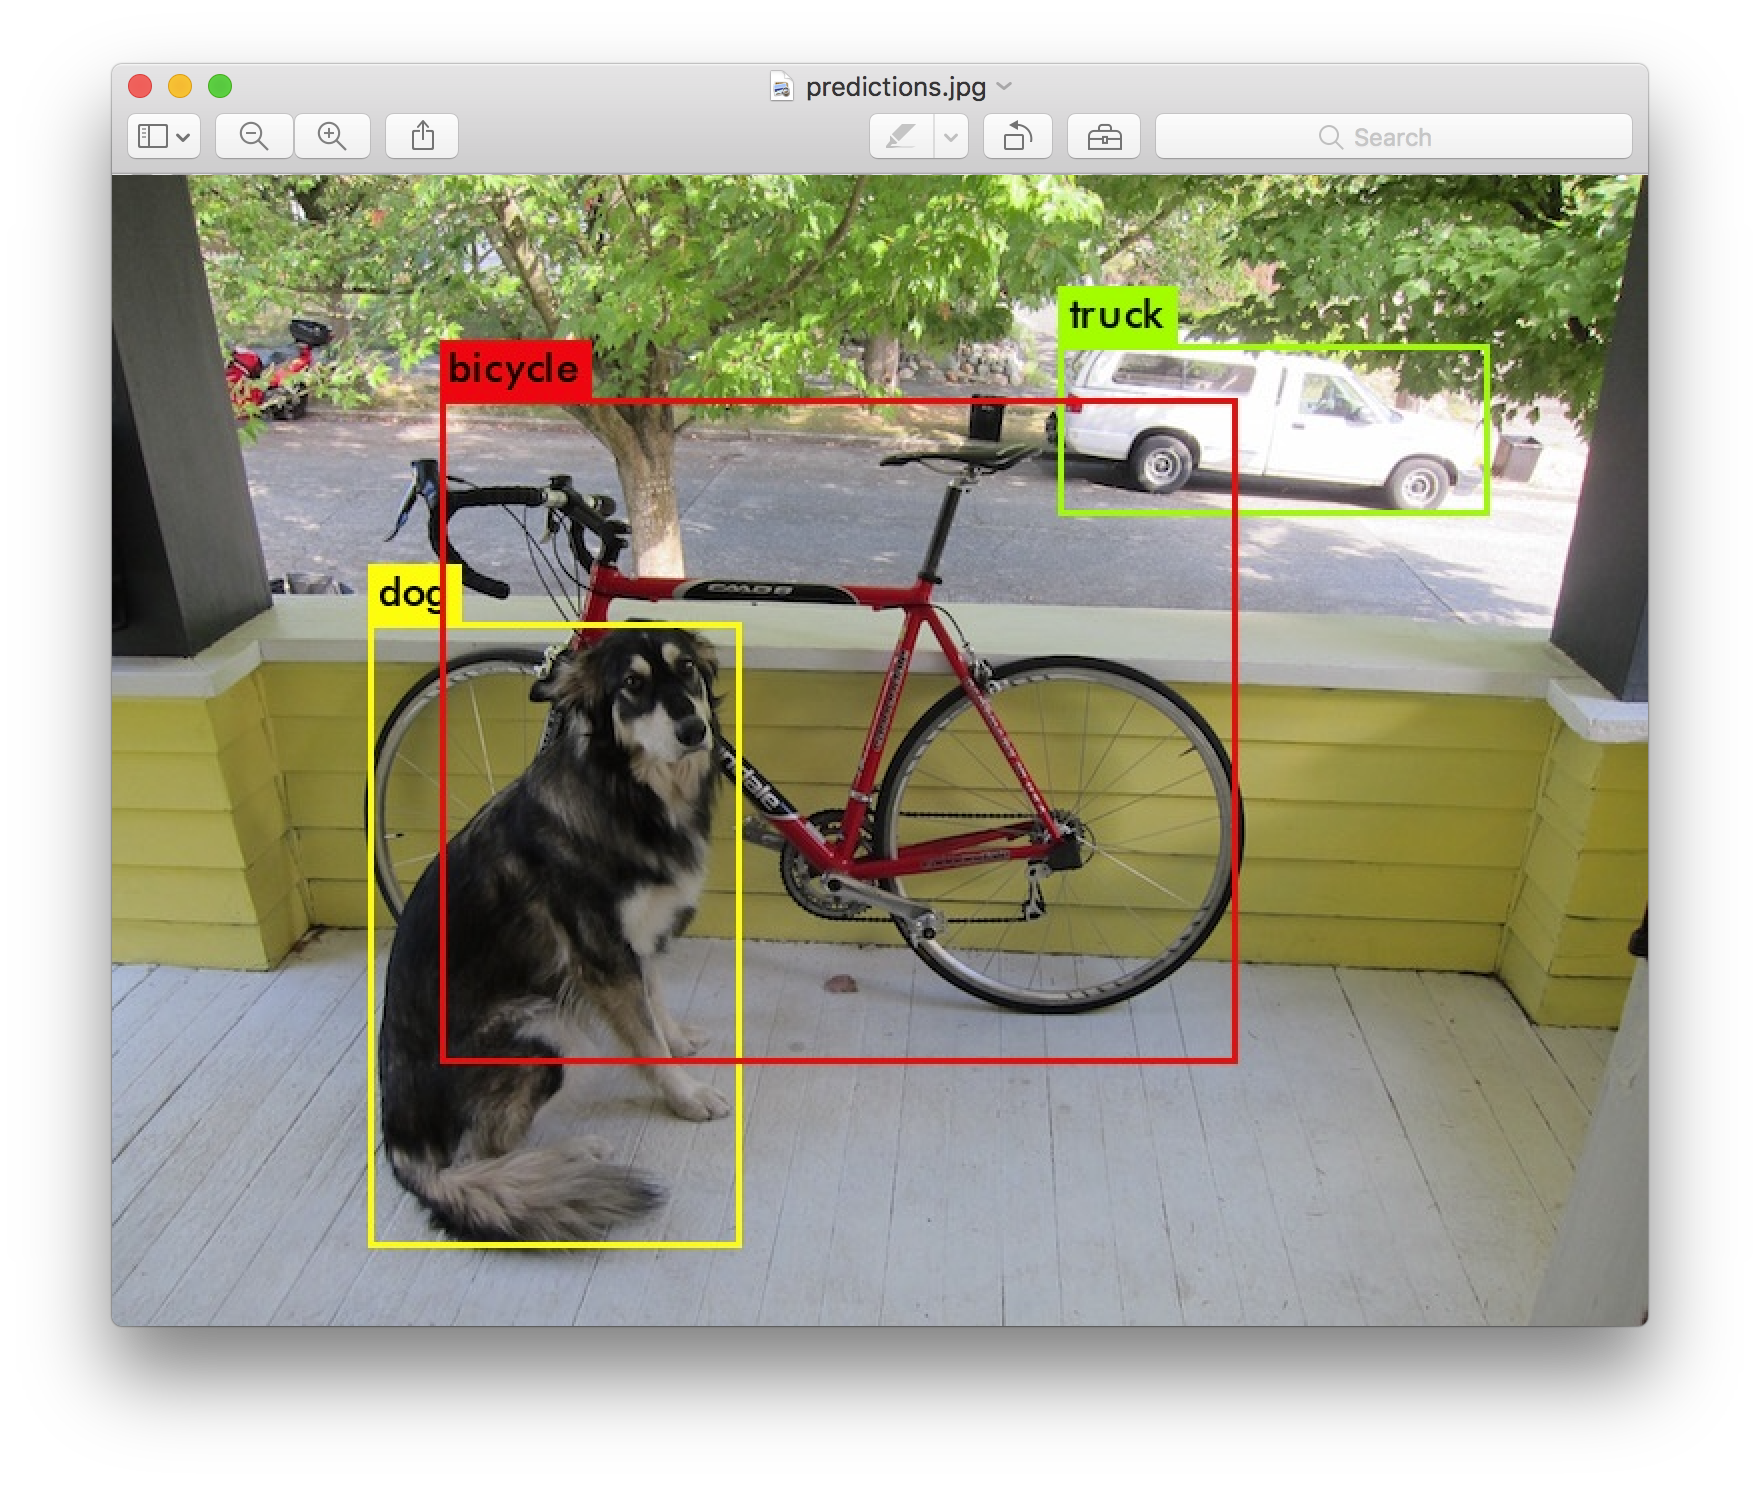
\includegraphics[scale=0.2]{../pdf/yolo.png}
        \caption{YOLO效果图}
        \label{}
    \end{figure}
    \subsection{LeNet-5}
    LeNet-5是一种用于手写体识别的卷积神经网络,是CNN领域五大经典模型之一。该网络虽小,但包含了深度学习的基本模块,如卷积层、池化层、全连接层,是其他CNN模型的基础,因此本文最后使用该模型进行测试。
    \begin{table}[h] %开始一个表格environment,表格的位置是h,here。  
        \centering
        \caption{LeNet-5 模型结构} %显示表格的标题  
        \begin{tabular}{l|l} %设置了每一列的宽度,强制转换。  
        \hline  
        Lenet-5 layers & 描述 \\
        \hline %画一个横线,下面的就都是一样了,这里一共有4行内容  
        Layer1[Conv] & Input: $32*32*1$ \  Filter: $5*5*6, stride=1$ \  Output: $28*28*6$ \\
        \hline  
        Layer2[Pooling] & Input: $28*28*6$ \  Filter: $2*2*6, stride=2$ \  Output: $14*14*6$ \\
        \hline  
        Layer3[Conv] & Input: $14*14*6$ \  Filter: $5*5*16, stride=1$ \  Output: $10*10*16$ \\
        \hline  
        Layer4[Pooling] & Input: $10*10*16$ \  Filter: $2*2*16, stride=2$ \  Output: $5*5*16$ \\
        \hline  
        Layer5[Fully Connect] & $400*120$ \\
        \hline  
        Layer6[Fully Connect] & $120*84$ \\
        \hline  
        Layer7[Fully Connect] & $84*10$  \\
        \hline  
        \end{tabular}  
    \end{table}


\section{本章小结}
本章首先对采用的开发工具进行了简要的阐述,其次举例介绍了目前使用较为广泛的异构处理器ZYNQ和RISC-V,最后介绍了利用CNN进行目标识别和图像识别的典型网络。

% \subsection{二级节标题}

% \subsubsection{三级节标题}

% \paragraph{四级节标题}

% \subparagraph{五级节标题}

% \section{脚注}

% Lorem ipsum dolor sit amet, consectetur adipiscing elit, sed do eiusmod tempor
% incididunt ut labore et dolore magna aliqua. Ut enim ad minim veniam, quis
% nostrud exercitation ullamco laboris nisi ut aliquip ex ea commodo consequat.
% Duis aute irure dolor in reprehenderit in voluptate velit esse cillum dolore eu
% fugiat nulla pariatur. Excepteur sint occaecat cupidatat non proident, sunt in
% culpa qui officia deserunt mollit anim id est laborum.
% \footnote{This is a long long long long long long long long long long long long
% long long long long long long long long long long footnote.}
